% -*- coding: utf-8 -*-
\documentclass[UTF8]{ctexart}

\title{\heiti \LaTeX 初学}
\author{\kaishu xuan}
\date{\today}

\bibliographystyle{plain}
\newtheorem{thm}{定理}
\usepackage{graphicx}
\usepackage{amsmath}
\usepackage[format=hang,font=small,textfont=it]{caption}
\usepackage[nottoc]{tocbibind}


\begin{document}

\maketitle
\newenvironment{myquote}{\begin{quote}\kaishu\zihao{-5}}{\end{quote}}
\newcommand{\degree}{^\circ}


\begin{abstract}
刚开始学\LaTeX,如果学习不是为了装逼,那一切将毫无意义。
\end{abstract}
\tableofcontents
\section{勾股定理在古代}
西方称勾股定理为毕达哥拉斯定理,将勾股定理的发现归功于公元前 6 世纪的毕达哥拉斯学派\cite{Kline}。该学派得到了一个法则,可以求出可排成直角三角形三边的三元数组。毕达哥拉斯学派没有书面著作,该定理的严格表述和证明则见于欧几里得\footnote{欧几里得,约公元前330-275年。}《几何原本》的命题 47:“直角三角形斜边上的正方形等于两直角边上的两个正方形之和。”证明是用面积做的。
我国《周髀算经》载商高(约公元前12世纪)答周公问:
\begin{myquote}
勾广三,股修四,经隅五。
\end{myquote}
又载陈子(约公元前7--6世纪)答荣方问:
\begin{myquote}
若求邪至日者,以日下为勾,日高为股,勾股各自乘,并而开方除之,得邪至日。
\end{myquote}
都较古希腊更早。后者已经明确道出勾股定理的一般形式。图\ref{fig:gougu}是我国古代对勾股定理的一种证明\cite{quanjing}。 
\begin{figure}[ht]
  \centering
  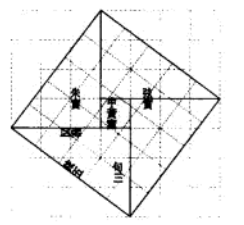
\includegraphics[width=3cm]{gougu.png}
  \caption {\kaishu\zihao{-5} 宋赵爽在《周髀算经》注中做的弦图(仿制),该图给出了勾股定理的一个极具对称美德证明。}
  \label{fig:gougu}
\end{figure}


\section{勾股定理的近代形式}
勾股定理可以用现代语言表述如下:
\begin{thm}[勾股定理]
直角三角形斜边的平方等于两腰的平方和。
可以用符号语言表述为:设直角三角形ABC,其中\angle C=$90\degree$,则有
\begin{equation} \label{eq:gougu}
AB^2 = BC^2 + AC^2
\end{equation}
\end{thm}

满足式\eqref{eq:gougu}的整数称为\emph{勾股数}。第1节所说毕达哥拉斯学派得到的三元数组就是勾股数。下表列出一些较小的勾股数:
\begin{table}[h]
\begin{tabular}{|rrr|}
\hline
直角边 $a$ & 直角边 $b$ & 斜边 $c$\\
\hline
3 &  4 & 5\\
5 &  12&  13\\
\hline
\end{tabular}%
\qquad
($a^2 + b^2 = c^2$)
\end{table}
\nocite{Shiye}
\bibliography{math}

\end{document}